\documentclass[12pt,twoside,book]{article}
\usepackage{docmute}

\input{../settings}

\begin{document}

%%%%%%%%%%%%%%%%%%%%%%%%%%%%%%%%%%%%%%%%%%%%%%%%%%%%%%%%%%%%%%%%%%%%%%%%%%%%%%%
\section{Direct collider search of WIMPs}
\setcounter{equation}{0}
\label{sec:direct}
%%%%%%%%%%%%%%%%%%%%%%%%%%%%%%%%%%%%%%%%%%%%%%%%%%%%%%%%%%%%%%%%%%%%%%%%%%%%%%%

\vskip 0.1in

In this section, we review the production of $\mathrm{TeV}$-scale WIMPs and search for their signals using the collider experiment.
In particular, we will summarize the current bounds for WIMPs obtained at the large hadron collider (LHC) and future bounds expected at the future planned $100\,\mathrm{TeV}$ colliders such as the hadron option of the future circular collider (FCC-hh) \cite{Benedikt:2651300} and the super proton-proton collider (SPPC) \cite{CEPC-SPPCStudyGroup:2015csa, CEPC-SPPCStudyGroup:2015esa}.
In Sec.~\ref{sec:wimp_production}, we discuss the dominant production processes of WIMPs at a hadron collider.
In Sec.~\ref{sec:disappearing_track} and \rem{???}, we review \rem{two???} different methods for the signal identification, the disappearing track search and mono-jet search \rem{???}, and summarize the current and future bounds.


%%%%%%%%%%%%%%%%%%%%%%%%%%%%%%%%%%%%%%%%%%%%%%%%%%%%%%%%%%%%%%%%%%%%%%%%%%%%%%%
\subsection{WIMP production}
\label{sec:wimp_production}
%%%%%%%%%%%%%%%%%%%%%%%%%%%%%%%%%%%%%%%%%%%%%%%%%%%%%%%%%%%%%%%%%%%%%%%%%%%%%%%

There are two relevant processes both of which significantly contribute to the WIMP production cross section.
The pair production via electroweak interaction is a universal process that can be considered for any WIMP considered in this thesis.
The decay of colored particles may also be efficient particularly for the MSSM.
In this subsection, we will review these two in order.


\subsubsection*{Pair production via electroweak interaction}

\begin{figure}[b]
  \centering
  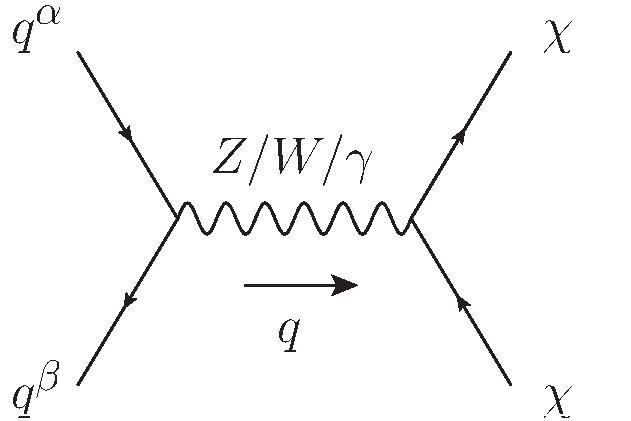
\includegraphics[width=0.4\hsize]{WIMP_production.pdf}
  \caption{WIMP pair production process at the hadron collider.}
  \label{fig:wimp_production}
\end{figure}

Since all the WIMPs considered here possess non-zero $SU(2)_L$ and $U(1)_Y$ charges, they can be directly produced via electroweak interaction at the hadron collider as shown in Fig.~\ref{fig:wimp_production}.
\footnote{
  All the Feynman diagrams in this thesis are drawn with the public code \texttt{JaxoDraw-2.1} \cite{BINOSI20091709}, which is a graphical user interface that allows users to draw Feynman diagrams intuitively and export them in the \texttt{eps} format with the help of the (modification of) \texttt{axodraw} style file for \LaTeX \cite{VERMASEREN199445}.
  Under the environment of macOS Mojave, it apparently fails to start, but one can still execute it by looking inside the application and start the Java executable file \texttt{jaxodraw-2.1-0.jar} directly.
  We would like to thank the authors for providing the best tools to write the thesis with.
  \rem{Where is the first place of Feynman diagrams?}
}
In the figure, $q^\alpha$ and $q^\beta$ denote the partons (namely, one of quarks or gluon) of the incident protons relevant for the process, while $\chi$ denotes the WIMP and $q$ is the momentum transfer.
Assuming the WIMP to be a $SU(2)_L$ $n$-plet with $U(1)_Y$ charge $Y$ and the mass $m_\chi$, this process is well described by the effective lagrangian
\footnote{
  In this subsection, we neglect the small mass difference among different components in the multiplet $\chi$ described in Sec.~\ref{sec:disappearing_track}.
  This approximation is valid since the mass difference is by far smaller than $m_\chi$ and has only a tiny effect on the production process.
}
\begin{align}
  \mathcal{L} &= \mathcal{L}_{\mathrm{SM}} + (D^\mu \chi)^\dagger (D_\mu \chi) - m_\chi^2 \chi^\dagger \chi &
  &\text{(complex scalar)}, \label{eq:lag_scalar}\\
  \mathcal{L} &= \mathcal{L}_{\mathrm{SM}} + \bar{\chi} (i \Slash{D} - m_\chi) \chi &
  &\text{(Dirac fermion)}, \label{eq:lag_fermion}
\end{align}
with $\mathcal{L}_{\mathrm{SM}}$ being the SM lagrangian, while the covariant derivative is given by
\begin{align}
  D_\mu \equiv \partial_\mu - i g_2 \Slash{W}^a T_n^a - i g_1 Y \Slash{B},
\end{align}
where $T_n^a$ ($a=1,2,3$) are $n$-dimensional representation matrices of $SU(2)_L$.
Note that when $\chi$ is a real scalar (Majorana fermion) with $Y=0$, the terms with $\chi$ in Eq.~\eqref{eq:lag_scalar} (Eq.~\eqref{eq:lag_fermion}) should be devided by two.

For the calculation, we neglect the effect of the electroweak symmetry breaking, which is valid because we are interested in the high-energy collision with the parton-level center-of-mass (CM) energy $\sqrt{s'} \equiv \sqrt{q^2} \gtrsim \mathrm{TeV}$.
Then, we consider the process in the CM frame and estimate the parton-level differential cross section as
\begin{align}
  \left. \frac{d \sigma_{\alpha \beta}}{d \sqrt{s'} d \Omega} \right|_{\text{CM}}
  &= \frac{C_{\alpha \beta}}{8 s'} \left( 1 - \frac{4 m_\chi^2}{s'} \right)^{3/2} \sin^2 \theta
  & &(\text{complex scalar}) \label{eq:parton_cross_section_scalar} \\
  \left. \frac{d \sigma_{\alpha \beta}}{d \sqrt{s'} d \Omega} \right|_{\text{CM}}
  &= \frac{C_{\alpha \beta}}{4 s'} \sqrt{1 - \frac{4 m_\chi^2}{s'}}
  \left[ 1 + \frac{4 m_\chi^2}{s'} + \left( 1 - \frac{4 m_\chi^2}{s'} \right) \cos^2 \theta \right]
  & &(\text{Dirac fermion}), \label{eq:parton_cross_section_fermion}
\end{align}
where $\theta$ is the angle between the momentum of the initial parton $q_a$ and that of one of the final state WIMPs.
These expressions are valid only when the center of mass energy exceeds the production threshold, $\sqrt{s'} > 2m_\chi$.
Note also that these expressions represent inclusive cross sections, \textit{i.e.}, the total cross section for the production of any component of the WIMP multiplet $\chi$.
The coefficient $C_{\alpha \beta}$ consists of contributions from $U(1)_Y$ and $SU(2)_L$ gauge bosons,
\footnote{
  There is no contribution from the interference term between $U(1)_Y$ and $SU(2)_L$ contributions, since it is proportional to $\mathrm{Tr} (T^a_n) = 0$.
}
\begin{align}
  C_{\alpha \beta} = c_{1 \alpha \beta} Y^2 \alpha_1^2
  + c_{2 \alpha \beta} I(n) \alpha_2^2,
\end{align}
with $I(n)$ being the Dynkin index for the $n$-dimensional representation given by
\begin{align}
  I(n) \equiv \frac{n^3-n}{12},
  \label{eq:dynkin}
\end{align}
which is normalized so that $I(2) = 1/2$.
The explicit form of $c_{1 \alpha \beta}$ and $c_{2 \alpha \beta}$, which are sizes of the couplings between partons of our choice and gauge bosons, can be expressed using the $U(1)_Y$ charge for a parton $Y_\alpha$ and the $SU(2)_L$ reducible 13-dimensional representation matrices for partons $T^a_{\alpha \beta}$ as
\begin{align}
  c_{1 \alpha \beta} &= Y_\alpha^2 \delta_{\alpha \beta},\\
  c_{2 \alpha \beta} &= \sum_a \left| T^a_{\alpha \beta} \right|^2.
\end{align}
Recalling that $\alpha_1 < \alpha_2$ and that we often consider the WIMPs with large $n$ and moderate $Y$, the WIMP production cross section grows as $n^3$ for larger multiplets according to Eq.~\eqref{eq:dynkin}.

In the reality, the initial state of the hadron collider is not the individual partons but two protons.
To obtain the cross section for the two protons initial state, we rely on the parton distribution function (PDF), which expresses the fraction of the partons with some given momentum in each accelerated proton.
Let $f_a (x)$ ($0 < x < 1$) be the PDF for a given parton $a$ inside a proton with momentum $p^\mu$.
$f_a (x)$ can be interpreted as a probability distribution to find the parton $\alpha$ with momentum $x p^\mu$, so we have a relationship
\begin{align}
  \sum_\alpha \int_0^1 dx \, x f_\alpha (x) = 1,
\end{align}
associated with the total momentum conservation, and
\begin{align}
  \int_0^1 dx \, \left[ f_d (x) - f_{\bar{d}} (x) \right] &= 1,\\
  \int_0^1 dx \, \left[ f_u (x) - f_{\bar{u}} (x) \right] &= 2,
\end{align}
from the composition of the proton.
Using the PDF, the cross section for the process of interest at the hadron collider is evaluated as
\begin{align}
  \frac{d \sigma}{d \sqrt{s'} d \Omega} =
  \sum_{\alpha, \beta} \int_0^1 dx_1 dx_2 \, f_\alpha (x_1) f_\beta (x_2) \delta \left( s' - s x_1 x_2 \right)
  \left. \frac{d \sigma_{\alpha \beta}}{d \Omega} \right|_{\text{lab}},
\end{align}
where $\sqrt{s}$ is the CM energy of the proton-proton collision.
Note that the cross section in the integrand is a function of $x_1$ and $x_2$, which is obtained by performing the appropriate Lorentz transformation to $\left. d \sigma_{\alpha \beta} / d \Omega\, \right|_{\text{CM}}$.
\rem{Comment on factorization scale?}

\begin{figure}[t]
  \centering
  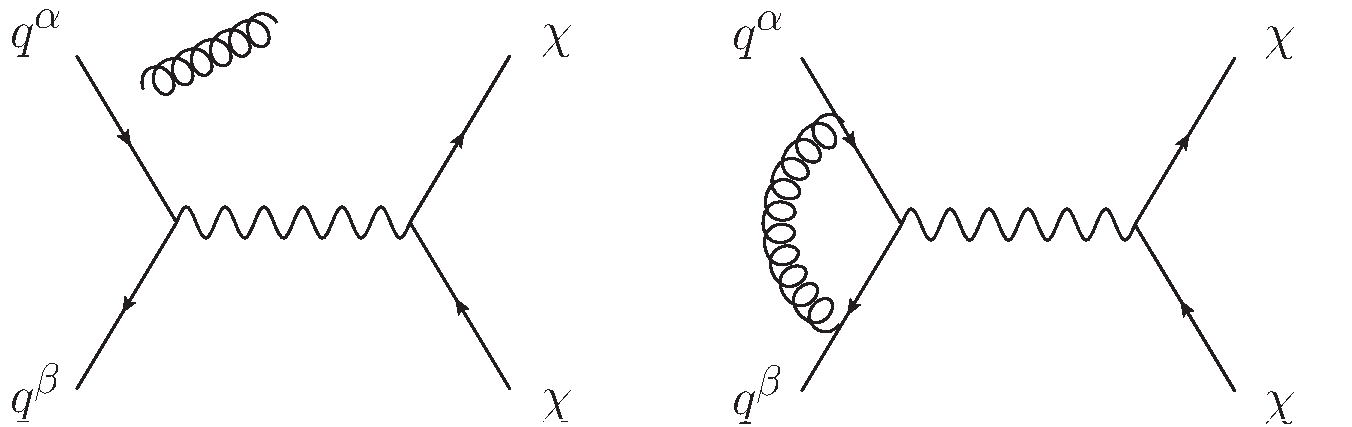
\includegraphics[width=0.8\hsize]{WIMP_production_NLO.pdf}
  \caption{Example of NLO QCD contributions to the WIMP pair production process.}
  \label{fig:WIMP_production_NLO}
\end{figure}

Hadron colliders have several more features related to the strong interaction of quantum chromodynamics (QCD).
Firstly, the next-to-leading order (NLO) QCD contribution to each process is not necessarily negligible.
For the WIMP pair production, the real and virtual emission of a gluon shown in the left and right panels of Fig.~\ref{fig:WIMP_production_NLO}, respectively, give the NLO QCD contributions, which will also be taken into account from now on.
In particular, when the large transverse momentum is important for the phenomenology of our concern, such as the case in Sec.~\rem{???}, the real emission of a gluon with sizable transverse momentum significantly modifies the calculation.
Secondly, all the colored particles in the initial, intermediate, and final states should be accompanied with numbers of soft emissions of gluons, which is the phenomena so-called the parton shower.
In practice, there is a difficulty caused by the partial overlap of the gluon phase space between the one-gluon emission cross section considered as an NLO QCD effect and the same considered as the parton shower.
To avoid this overlap, we often perform the matching procedure, in which we set some merging energy scale by hand and include the contribution to the cross section with gluon energy above (below) the scale only from the NLO QCD (parton shower) calculation.
Finally, the colored particles in the final states should eventually be confined, which is called the hadronization, and observed as some energetic and collimated sprays of hadrons, which as a whole is called jets.

In the following, we perform the numerical calculation, taking account of all the above complexities.
For this purpose, we make use of the Monte Carlo generator \texttt{MadGraph5 aMC@NLO (v2.6.3.2)} \cite{Alwall:2011uj,Alwall:2014hca} with the successive use of \texttt{Pythia8} \cite{Sjostrand:2014zea} for the parton shower, hadronization, and matching and \texttt{Delphes (v3.4.1)} \cite{deFavereau:2013fsa} for the detector simulation, including the definition of jets as observed objects.
We use the so-called MLM-style matching \cite{Mangano:2006rw} with the merging scale of $67.5\,\mathrm{GeV}$ and \texttt{NNPDF2.3QED} with $\alpha_3 (M_Z) = 0.118$ \cite{Ball:2013hta} as a canonical set of PDFs.
% For the renormalization and factorization scales, we adopt the default values of MadGraph5 aMC@NLO, \textit{i.e.}, the central $m^2_T$ scale after $k_T$-clustering of the event.

\begin{table}[t]
  \centering
  \begin{tabular}{c|cccc}
    WIMP name & Higgsino & Wino & $5$-plet Majorana fermion & $5$-plet real scalar \\ \hline
    $\sigma_{\mathrm{LO}}$ $[\mathrm{fb}]$ & 15 & 52 & \rem{???} & \rem{???} \\
    $\sigma_{\mathrm{NLO}}$ $[\mathrm{fb}]$ & 17 & 60 & \rem{???} & \rem{???} \\ \hline
    $K$-factor & 1.15 & 1.15 & &
  \end{tabular}
  \caption{
    Table of pair production cross sections of several types of WIMPs.
    The CM energy $\sqrt{s} = 100\,\mathrm{TeV}$ is assumed and WIMP masses are set to be $1\,\mathrm{TeV}$.
  }
  \label{tab:cross_section_WIMPs}
\end{table}

In Table~\ref{tab:cross_section_WIMPs}, we list the production cross sections of various WIMPs via a weak gauge boson exchange at a $\sqrt{s} = 100\,\mathrm{TeV}$ hadron collider.
As for the WIMP mass, we use the common value $m = 1\,\mathrm{TeV}$ to compare the cross sections among different choice of quantum numbers.
$\sigma_{\mathrm{LO}}$ and $\sigma_{\mathrm{NLO}}$ denote the production cross sections without and with the NLO QCD correction, respectively, while the last line is the so-called $K$-factor defined as $K = \sigma_{\mathrm{NLO}} / \sigma_{\mathrm{LO}}$.
From the table, by paying attention to the factor two difference in degrees of freedom between the Dirac (Higgsino) and Majorana (Wino and $5$-plet) fermions, we can roughly see the dependence of the cross section on the $SU(2)_L$ charge $\sigma \propto n^3$.
\rem{Cross section to neutral Higgsino seems missing}

\begin{table}[t]
  \centering
  \begin{tabular}{c|cccc}
    Wino mass $\mathrm{[TeV]}$ & 1.0 & 1.5 & 2.0 & 2.9 \\ \hline
    $\sigma_{\mathrm{LO}}$ $[\mathrm{fb}]$ & 52 & 12 & 4.0 & 0.86\\
    $\sigma_{\mathrm{NLO}}$ $[\mathrm{fb}]$ & 60 & 15 & 4.7 & 1.0 \\ \hline
    $K$-factor & 1.15 & 1.20 & 1.19 & 1.21
  \end{tabular}
  \caption{
    Table of pair production cross sections of Wino with several choice of masses.
    The CM energy $\sqrt{s} = 100\,\mathrm{TeV}$ is assumed.
  }
  \label{tab:cross_section_Wino_mass}
\end{table}

In Table \ref{tab:cross_section_Wino_mass}, we also show the mass dependence of the Wino pair production cross section.
For heavier mass, wider range of $\sqrt{s'}$ is below the production threshold $2 m_{\chi}$ or accompanied with a small suppression factor $(1-4 m_\chi^2 / s')^{1/2}$ as shown in Eq.~\eqref{eq:parton_cross_section_fermion}, and the cross section becomes significantly smaller.
However, values in the tables still denote that plenty of well-motivated WIMP DM candidates, such as $1\,\mathrm{TeV}$ Higgsino and $2.9\,\mathrm{TeV}$ Wino, are produced at, for example, the $30\,\mathrm{ab}^{-1}$ option of the FCC-hh.

\begin{figure}[t]
  \centering
  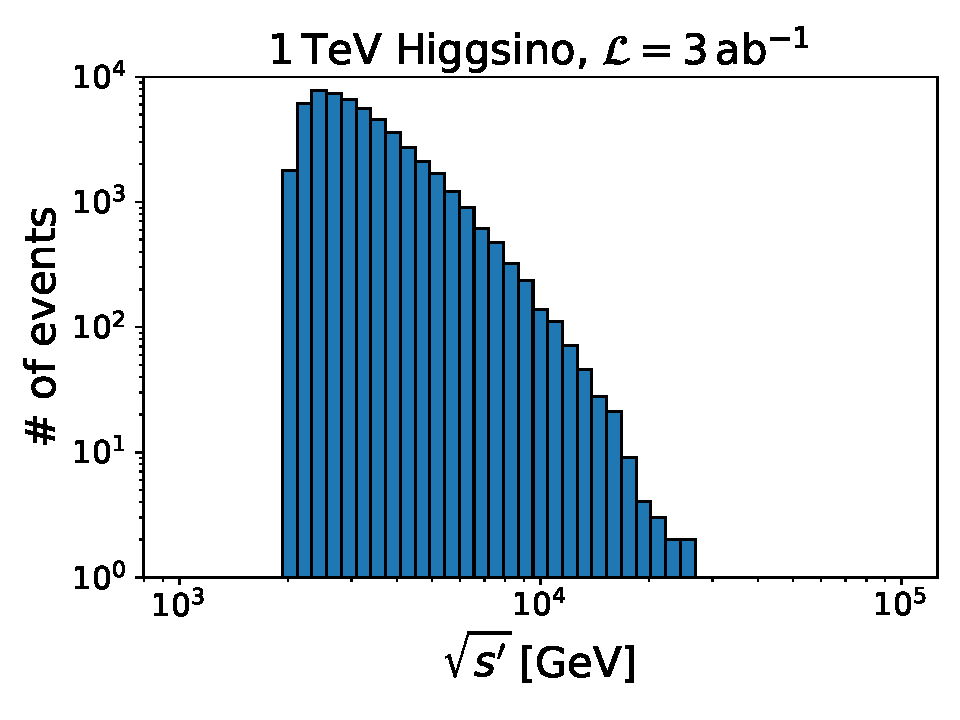
\includegraphics[width=0.48\hsize]{invariant_mass_Higgsino.pdf}
  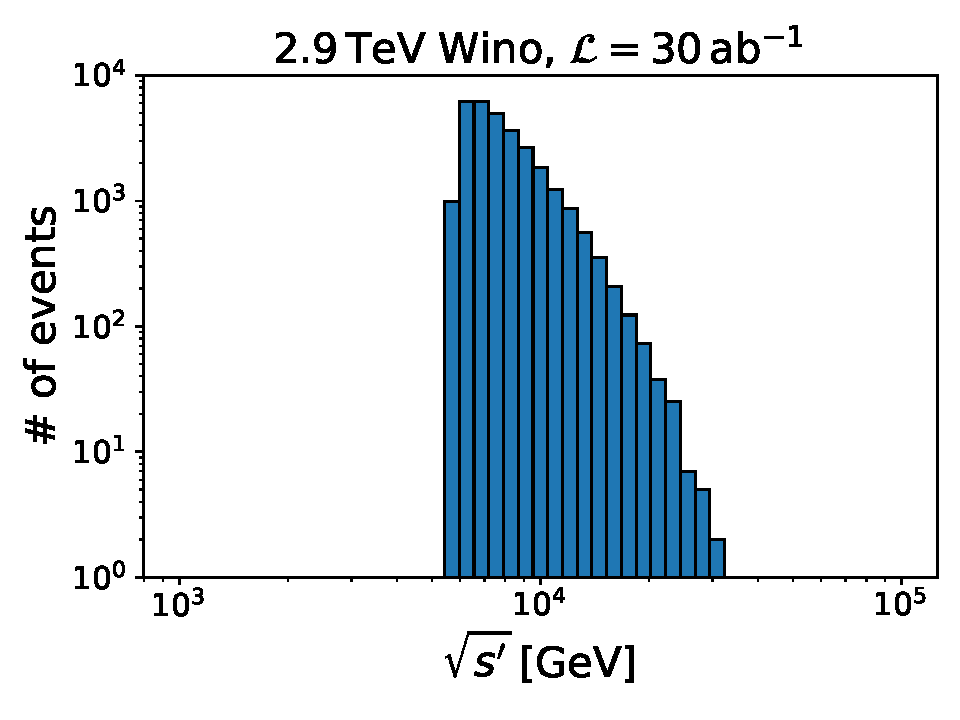
\includegraphics[width=0.48\hsize]{invariant_mass_Wino.pdf}
  \caption{
    Histogram of the $\sqrt{s'}$ distribution for $\sqrt{s} = 100\,\mathrm{TeV}$.
    \textit{Left:} Production of $1\,\mathrm{TeV}$ Higgsino at $\mathcal{L} = 3\,\mathrm{ab}^{-1}$.
    \textit{Right:} Production of $2.9\,\mathrm{TeV}$ Wino at $\mathcal{L} = 30\,\mathrm{ab}^{-1}$.}
  \label{fig:invariant_mass}
\end{figure}

In Fig.~\ref{fig:invariant_mass}, we show the $\sqrt{s'}$ distribution for the pair production process at a $\sqrt{s} = 100\,\mathrm{TeV}$ collider.
Left and right figures correspond to the production of $m_\chi = 1\,\mathrm{TeV}$ Higgsino at the integrated luminosity $\mathcal{L} = 3\,\mathrm{ab}^{-1}$ and of $m_\chi = 3\,\mathrm{TeV}$ Wino at $\mathcal{L} = 30\,\mathrm{ab}^{-1}$, respectively.
At around $\sqrt{s'} \sim 2 m_\chi$, we clearly see the production threshold and the suppression effect $\sigma \propto (1-4 m_\chi^2 / s')^{1/2}$.
On the other hand, when $\sqrt{s'}$ becomes much larger than $2m_\chi$, we can see the correct behavior of the cross section, which decreses as $\sigma \propto (\sqrt{s'})^{-3}$ as Eq.~\eqref{eq:parton_cross_section_fermion} indicates.
Note that these properties are universal among several processes, including the dominant contribution \rem{Correct?} to the gluino pair production through the $s$-channel gluon exchange disscused in the next subsection, and the lepton pair production through via an electroweak gauge boson that is the main topics in Sec.~\rem{???}.

\rem{Histogram of angular dependence}

\rem{Is angular dependence affected by the Lorentz boost?}


\subsubsection*{Decay of colored particles}

In hadron colliders, particles with color charges have far more chance to be produced than non-colored particles.
When we consider the split SUSY or the anomaly mediation model reviewed in Sec.~\ref{sec:MSSM}, gluino tends to be relatively light, whose decay produces WIMPs.
Without fine-tuning of Higgsino and gaugino masses, gluino lifetime is sufficiently short and only its decay products are observed by the detectors.
Since all the SUSY particles finally decay into the LSP as described in Sec.~\ref{sec:MSSM}, the gluino production cross section can effectively be counted as the production cross section of WIMPs in these models.

\begin{table}[t]
  \centering
  \begin{tabular}{c|ccc}
    gluino mass $\mathrm{[TeV]}$ & 6.0 & 7.0 & 8.0 \\ \hline
    $\sigma(p p \to \tilde{g} \tilde{g})\, \mathrm{[fb]}$ & 7.9 & 2.7 & 1.0
  \end{tabular}
  \caption{Gluino pair production cross section at $\sqrt{s} = 100\,\mathrm{TeV}$.}
  \label{tab:gluino_pair}
\end{table}

Keeping the R-parity conservation in our mind, the dominant process accompanied with gluinos in these models is the gluino pair production.
In Table \ref{tab:gluino_pair}, we summarize the gluino pair production cross section for various gluino masses at $\sqrt{s} = 100\,\mathrm{TeV}$, taken from \cite{Asai:2019wst}.
The calculation is again performed using \texttt{MadGraph5 aMC@NLO} and only the LO QCD processes are considered.
The values in the table show that the gluino pair production process, dependeing on its mass, may give much larger cross section for the WIMP production than the purely electroweak processes described above.

\rem{Comment on AMSB $m_{3/2}$ and $L$ for the table?}


%%%%%%%%%%%%%%%%%%%%%%%%%%%%%%%%%%%%%%%%%%%%%%%%%%%%%%%%%%%%%%%%%%%%%%%%%%%%%%%
\subsection{Disappearing track search}
\label{sec:disappearing_track}
%%%%%%%%%%%%%%%%%%%%%%%%%%%%%%%%%%%%%%%%%%%%%%%%%%%%%%%%%%%%%%%%%%%%%%%%%%%%%%%

In the last section, we have checked the possibility that a large number of WIMPs are produced at hadron colliders.
On the other hand, the detection of produced WIMPs is not a straight-forward task, because there are huge background events with many charged and/or colored particles.
To reduce the background events and obtain the best possible reach for WIMPs, we consider several methods using typical properties for the WIMP signals, one of which is the disappering track signal described here.

As also mentioned in Sec.~\rem{DM??}, the spontaneous breaking of the electroweak symmetry leads to the mass splitting among an $SU(2)_L$ multiplet, leaving the charge neutral component as the lightest one.
As a result, the charged components of a multiplet, if produced, are unstable and eventually decay into the neutral component.
However, the mass splitting is so small in many cases that the typical flight length of the charged components is comparable to the detector size.
Such long-lived charged particles, which travel for a few $\mathrm{cm}$ and then decay into an invisible counterpart, can be detected as charged tracks disappearing at the middle.
They are very characteristic signals and can be used as the most efficient discriminator between the SM background and the WIMP signals.
In this section, we will describe what we have summarized above in more detail.


\subsubsection*{Lifetime of charged components}

Small mass difference of a WIMP allows the heavier charged component to decay into the neutral component and SM particles via a off-shell $W$ boson.
Depending on the size of the relevant mass difference $\Delta m$, there are several channels that contributes to the decay \cite{Chen:1995yu}.
For tiny $\Delta m < m_\pi$ with $m_\pi$ being the charged pion mass, $\chi^{+} \to \ell^{+} \nu_\ell \chi^0$ ($\ell = e, \mu$) are the unique decay modes.
Once $\Delta m$ exceeds $m_\pi$, the mode $\chi^{+} \to \pi^{+} \chi^0$ opens up and becomes the dominant one.
After $\Delta m \gtrsim 1\, \mathrm{GeV}$, final states with two and three pions start to give a sizable contribution, and the total decay rate asymptotes to that for $\chi^{+} \to q' \bar{q} \chi^0$.
For larger mass difference, the mode $\chi^{+} \to \tau^{+} \nu_\tau \chi^0$ may also be allowed.
As a whole, these decay modes determine the lifetime of a WIMP, which is typically long enough to be probed by experiments thanks to the small mass difference.

Let $\tau$ be the lifetime of the (singly) charged component of a WIMP, defined using the total decay rate $\Gamma$ as $\tau \equiv 1/\Gamma$.
Taking into account that a WIMP, if created at colliders with sufficiently high collision energy, has a velocity comparable to the speed of light $c$, $c \tau$ expresses the rough estimation of its flight length inside detectors.
For Higgsino with $m_\pi < \Delta m \lesssim 1\,\mathrm{GeV}$,
\footnote{
  We are not interested in Higgsino with $\Delta m \gtrsim 1\, \mathrm{GeV}$ here, since the corresponding flight length will be much shorter than $\mathcal{O} (1)\, \mathrm{cm}$, which is the scale of the detectors.
}
we can estimate \cite{Chen:1995yu,Thomas:1998wy}
\begin{align}
  c \tau \simeq 0.7\, \mathrm{cm}
  \left[ \left( \frac{\Delta m_{+}}{340\,\mathrm{MeV}} \right)^3
  \sqrt{1 - \frac{m_\pi^2}{\Delta m_{+}^2}} \right]^{-1},
\end{align}
where $\Delta m_{+} \equiv \Delta m_{+}^{\mathrm{tree}} + \Delta m_{+}^{\mathrm{rad}}$ with using Eqs.~\eqref{eq:Higgsino_delm_tree} and \eqref{eq:Higgsino_delm_rad}.
Since the mass difference for wino is a factor two smaller than Higgsino, we obtain a much longer flight length
\begin{align}
  c \tau \simeq 3.1\, \mathrm{cm} \left[
  \left( \frac{\Delta m}{165\, \mathrm{MeV}} \right)^3
  \sqrt{1 - \frac{m_\pi^2}{\Delta m^2}} \right]^{-1},
\end{align}
which gives $c\tau \simeq 5.8\,\mathrm{cm}$ for $\Delta m = 165\,\mathrm{MeV}$.
The same calculation applies to the MDMs with $n \geq 5$ and $\Delta m = 166\, \mathrm{MeV}$, resulting in somewhat shorter flight length that scales as $c \tau \sim 44\, \mathrm{cm} / (n^2 - 1)$ \cite{Cirelli:2005uq} due to the stronger interaction with $W$ bosons.
\rem{Scalar?}


\subsubsection*{Disappering track signal}

Once a long-lived charged component of WIMP is produced, it is detected by the trackers installed in the innermost part of the detectors for the case of ATLAS and CMS collaborations at the LHC.
For example, in the ATLAS setup, several tracking detectors are equipped cyrindrically around the beam line from the radius $r = 3\,\mathrm{cm}$ to $108\,\mathrm{cm}$.
The pixel detector spans the radius from $3\,\mathrm{cm}$ to $12\,\mathrm{cm}$, the strip semiconductor tracker (SCT) from $30\,\mathrm{cm}$ to $52\,\mathrm{cm}$, and the transition radiation tracker from $56\,\mathrm{cm}$ to $108\,\mathrm{cm}$.
In particular, pixel detectors are the most important for our discussion, which are composed of four layers, with the innermost one being the rescently equipped so-called the insertable B-layer \cite{Capeans:1291633, CERN-LHCC-2012-009, Abbott:2018ikt}.
To detect the charged track signal of a long-lived WIMP with the typical flight length of $\mathcal{O} (1)\, \mathrm{cm}$, they require the hit at every layer of the pixel detector and apply the SCT veto to search for the track signal disappearing in between $12\,\mathrm{cm} < r < 30\,\mathrm{cm}$.
As for the fake events within the SM, the SCT veto denies the possibility for a stable SM particle to mimic the signal.
However, there are two important sources of the fake track generated by hadrons/electrons and the so-called pile-up.

The first possibility with hadrons/electrons is a physical background caused by the interaction of hadrons with detector material or by the hard photon emission of electrons.
After these interactions, the orbit of a hadron/electron is bended and, if this secondary interaction point is between the pixel trackers and the SCT, two tracks in these two detectors are not identified with each other.
As a result, the first track in the pixel trackers seems to disappear in the middle, which mimics the true WIMP signals.
In the LHC, this type of background dominates and generates $\mathcal{O}(10$--$100)$ fake tracks for $\sqrt{s}=13\,\mathrm{TeV}$, $\mathcal{L} = 36.1\,\mathrm{fb}^{-1}$ (see Fig.~7 of \cite{Aaboud:2017mpt}).

On the other hand, for future hadron colliders, the second possibility of the fake track from the pile-up may be more and more important.
In hadron colliders, a bunch of protons are accelerated at the same time and two bunches ``collide'' with each other with some given frequency.
Since there are many protons inside a bunch, typically more than one collisions of two protons occur for each bunch crossing.
The average number of collisions per bunch crossing is often denoted as $\Braket{\mu}$ and the values of $\Braket{\mu} \sim 20$, $80$, and $200$ are expected for LHC Run-2, Run-3, and HL-LHC.
With this many collisions, there are a lot of collision products detected almost at the same time, which makes the signal significantly messy.
Then, among a huge number of hits on track detectros, several of them occasionally form a straight line in position and time, which is sometimes called the fake track.
Since this track is only a fake, it can easily pass the SCT veto and mimic the disappearing track signal of WIMPs.
In the real experiment, the rate for fake track reduces as we require more hits on trackers.
See the results below for a concrete estimation of the fake track rate at the FCC-hh.

\begin{figure}[t]
  \centering
  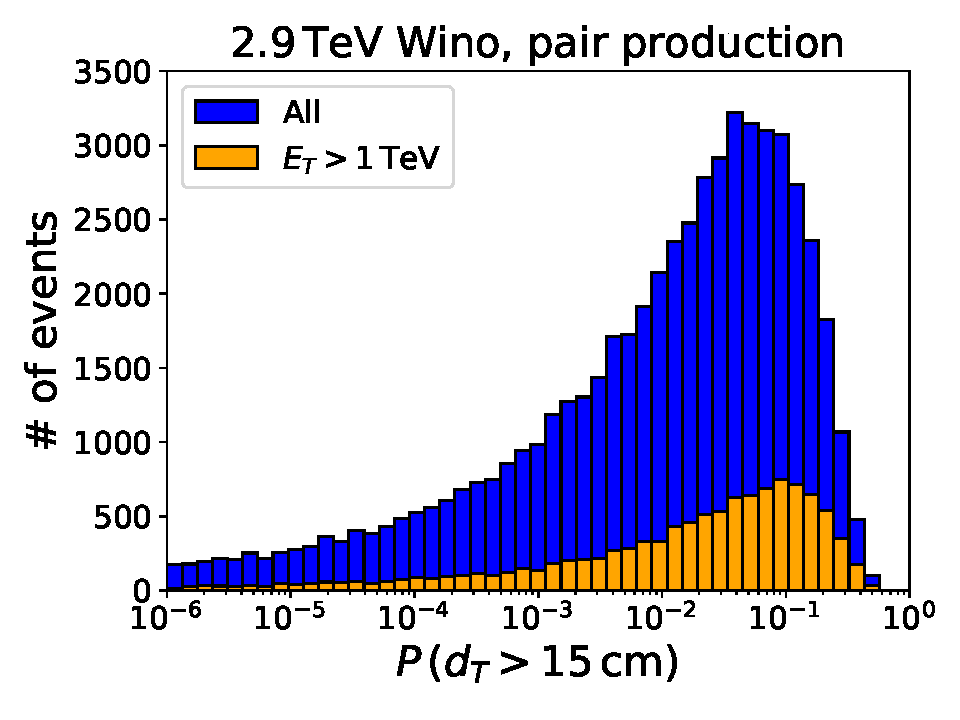
\includegraphics[width=0.5\hsize]{survival_probability.pdf}
  \caption{
    Distribution of the survival probability $P(d_T > 15\,\mathrm{cm})$ for $2.9\,\mathrm{TeV}$ Wino.
    The pair prodction process at $\sqrt{s}=100\,\mathrm{TeV}$ and $\mathcal{L} = 30\,\mathrm{ab}^{-1}$ is assumed.}
  \label{fig:survival_probability}
\end{figure}

From now on, we estimate how many events are expected at the FCC-hh.
Recalling that the detectors are installed in a cyrindrical geometry, the transverse distance $d_T$ of the WIMP flight measured from the beam line plays an important roll.
We can estimate the probability for $d_T$ to be larger than $d$ as
\begin{align}
  P(d_T > d) = \exp \left( -\frac{d}{\beta \gamma c \tau \sin\theta} \right),
  \label{eq:survival_probability}
\end{align}
where $\beta$ is the WIMP velocity, $\gamma \equiv (1-\beta^2)^{-1/2}$, and $\theta$ is the angle between the WIMP momentum and the beam line.
One of the implications of the above expression is that WIMPs with large transverse momentum have larger possibility to survive for a long time.
This enlarges the importance of considering the NLO (and higher order) QCD processes with real emission for the pair production.
Due to the hard emission of gluon, the produced pair of WIMPs is recoiled in an opposite direction, and WIMPs tend to have larger transverse momentum than the case without gluon emission.
It can be directly checked that, for $\sqrt{s}=100\,\mathrm{TeV}$, even the two-gluon emission process possesses non-negligible contribution to the simulation of the disappearing track search for WIMPs.

In Fig.~\ref{fig:survival_probability}, we show the distribution of $P(d_T > 15\,\mathrm{cm})$ (which is motivated by the FCC-hh detector setup assumed below) for the $2.9\,\mathrm{TeV}$ Wino, $\sqrt{s} = 100\,\mathrm{TeV}$, and $\mathcal{L} = 30\,\mathrm{ab}^{-1}$.
Here, we only consider the WIMP pair production process with upto one gluon emission as an example.
Note that $\tau \simeq 5.8\,\mathrm{cm}$ for this setup.
We can see that the increase in the probability by $\gamma$ and the decrease by $\beta$ and $\sin\theta$ roughly cancels with each other on average, resulting in a peak of the distribution at $P \sim 10^{-1} \sim \exp (-15\,\mathrm{cm} / \tau)$.
By summing the shown probabilities for all produced winos, we can obtain the expectation value $N_{15}$ for the number of winos with $d_T > 15\,\mathrm{cm}$.
We find $N_{15} \sim 2400$,
\footnote{
  In the real analysis, it may also be important to put a cut on the missing transverse energy $\Slash{E}_T$ to further reduce the number of background.
  If we require $\Slash{E}_T > 1\,\mathrm{TeV}$ as \cite{Asai:2019wst}, we expect smaller number of winos $N_{15} \sim 600$.
}
to which a lot of winos around and above the peak position $P \sim 10^{-1}$ significantly contribute.
Thus, we infer that we can detect the wino signal if we can suppress the number of background events to $\lesssim \mathcal{O}(10^5)$.
In the next subsection, we will see that this is the case for the FCC-hh and the parameter space for the wino DM candidate can fully be covered.

\begin{figure}[t]
  \centering
  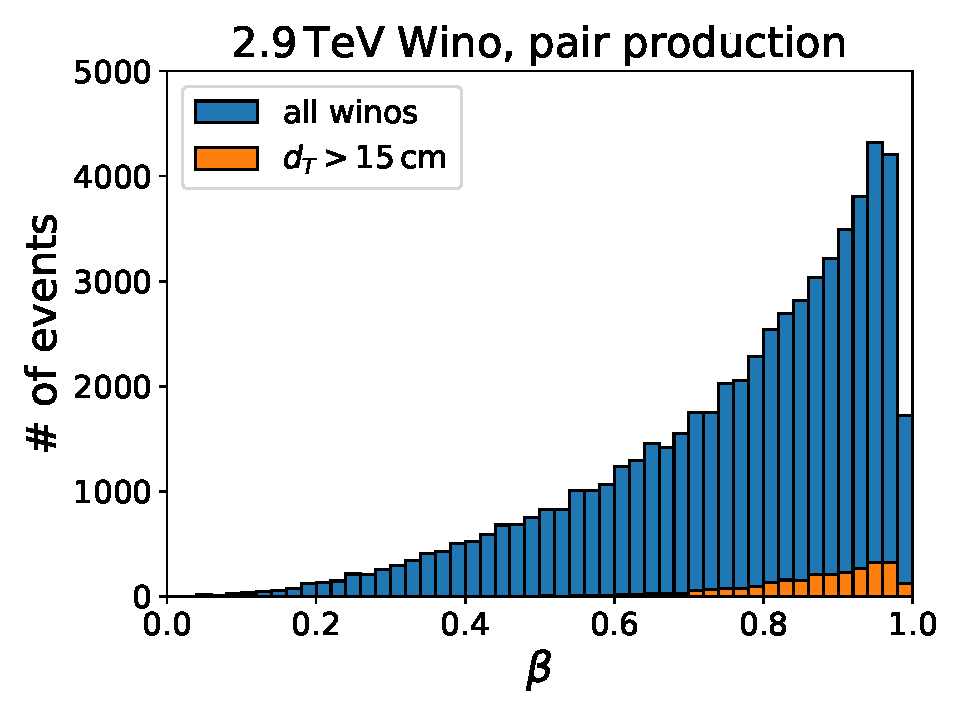
\includegraphics[width=0.5\hsize]{beta.pdf}
  \caption{
    Distribution of the Wino velocity $\beta$ for $2.9\,\mathrm{TeV}$ Wino.
    The pair prodction process at $\sqrt{s}=100\,\mathrm{TeV}$ and $\mathcal{L} = 30\,\mathrm{ab}^{-1}$ is assumed.
  }
  \label{fig:beta}
\end{figure}

In Fig.~\ref{fig:beta}, we show the distribution of the wino velocity $\beta$ for the same process.
The blue histogram shows the distribution of all winos, while the orange one shows that of winos with $d_T > 15\,\mathrm{cm}$, picked up according to the survival probability Eq.~\eqref{eq:survival_probability}.
As already seen in Fig.~\ref{fig:invariant_mass}, the center of mass energy of the two wino system distributes from a few to $\mathcal{O} (10) \,\mathrm{TeV}$, and many winos are highly boosted with $\beta \sim 1$.
Since a wino tends to fly for longer distance when it is more accelerated, some of boosted winos $\beta \gtrsim 0.6$ satisfy the requirement $d_T > 15\,\mathrm{cm}$.


\subsubsection*{Current constraints and future prospects}

The produced charged component of a WIMP is first detected by the trackers, which is equipped in the most inner part of detectors.
So far, the search is performed by both ATLAS \cite{Aaboud:2017mpt} and CMS \cite{Sirunyan:2018ldc} collborations.
Below, we will focus particularly on the ATLAS collaboration and discuss current constraints.

\begin{figure}[t]
  \centering
  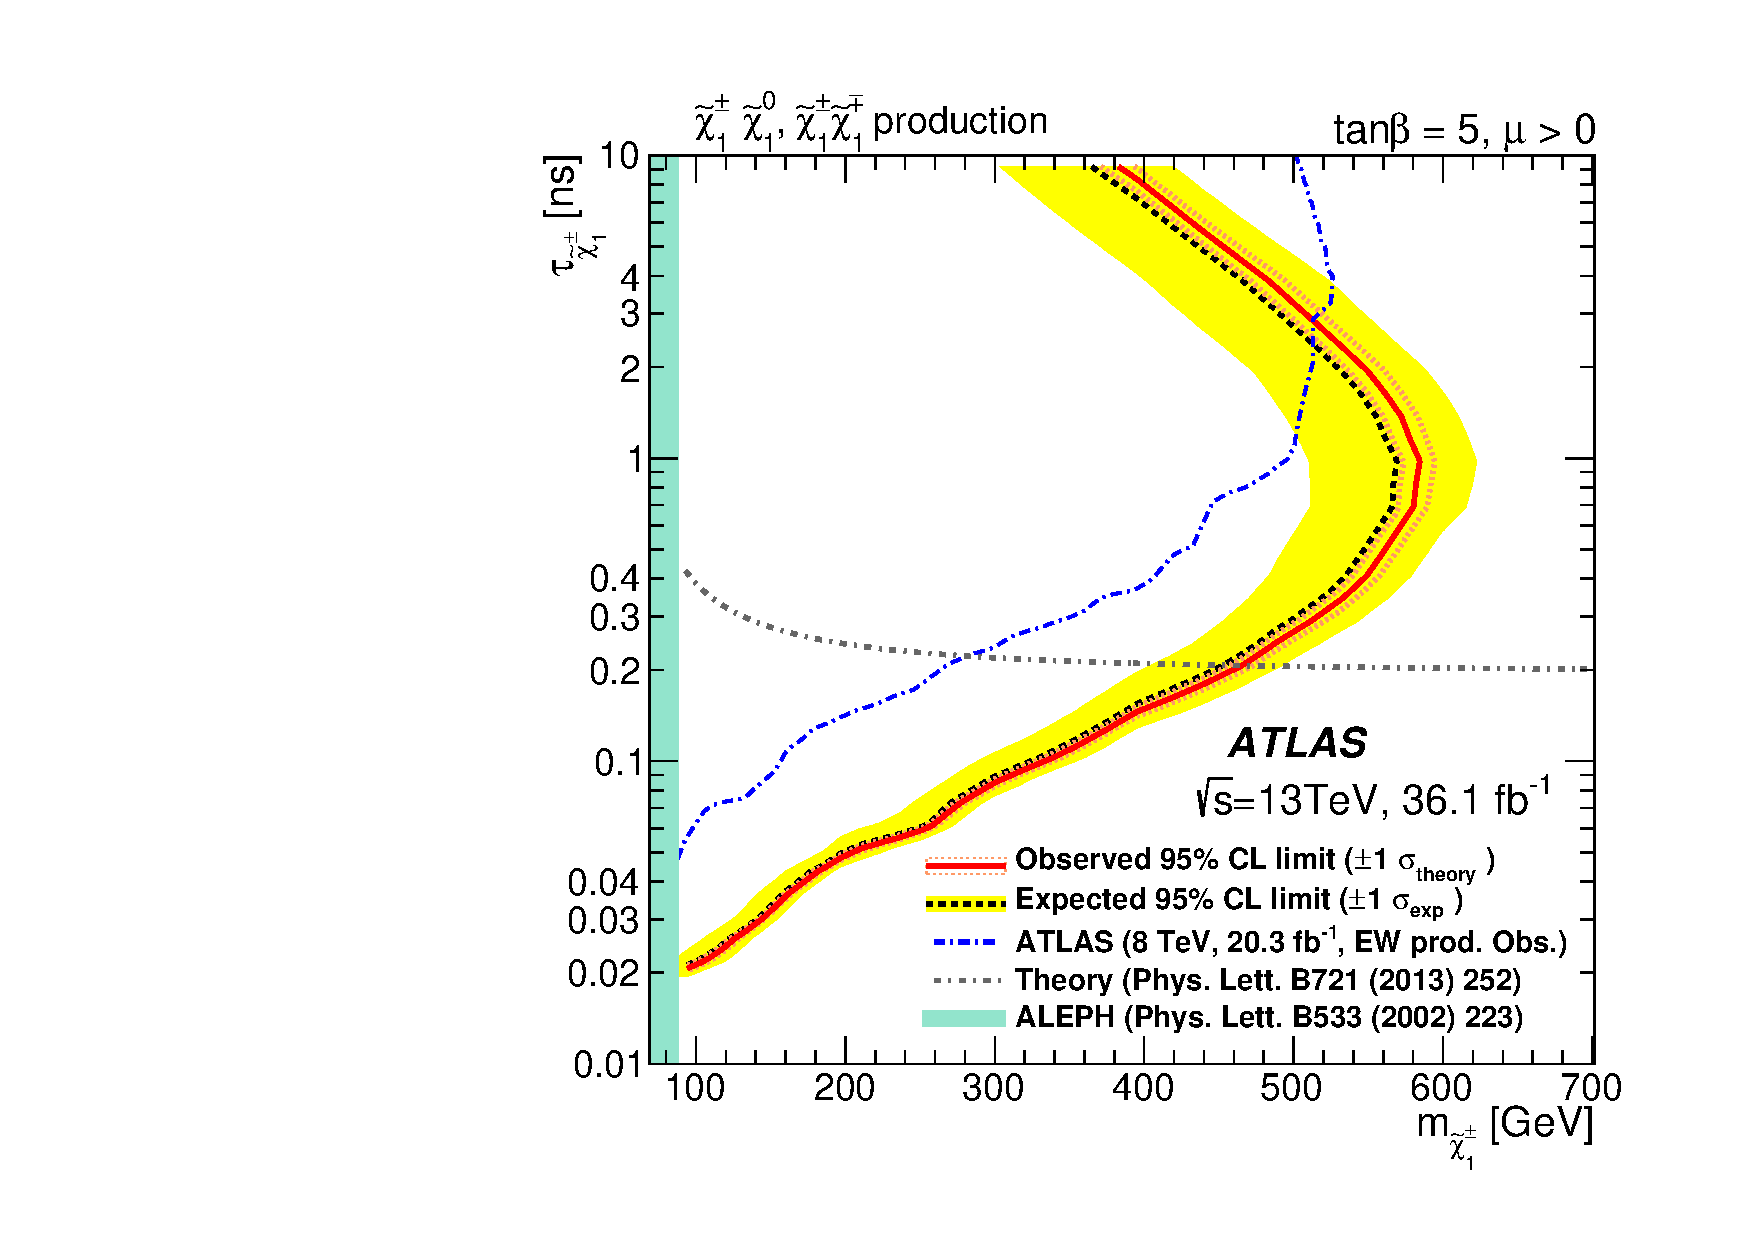
\includegraphics[width=0.5\hsize]{ATLAS_disappearing_track.pdf}
  \caption{Current status of the disappearing track search taken from \cite{Aaboud:2017mpt}.}
  \label{fig:ATLAS_disappearing_track}
\end{figure}

\begin{table}[t]
  \centering
  \begin{tabular}{c|ccc}
    WIMP & pure Higgsino & Wino & $5$-plet fermion \\ \hline
    Upper bound on $m_\chi$ & $120\, \mathrm{GeV}$ & $460\, \mathrm{GeV}$
    & $260\, \mathrm{GeV}$
  \end{tabular}
  \caption{
    Current upper bound for WIMP masses obtained from the disappearing track search shown in Fig.~\ref{fig:ATLAS_disappearing_track}.}
  \label{tab:disp_track_current}
\end{table}

In Fig.~\ref{fig:ATLAS_disappearing_track}, we show the result of the disappearing track search taken from \cite{Aaboud:2017mpt}.
The yellow band shows the current constraint on the WIMP mass and lifetime plane and the left part of the band is already excluded.
The sensitivity becomes weak when we consider $\tau \gtrsim 1\, \mathrm{ns}$ or $c \tau \gtrsim 30\, \mathrm{cm}$ due to the requirement of the SCT veto.
In the figure, the lifetime of Wino as a function of its mass is also shown by the black dot-dashed line.
It can be seen that the current contraint on Wino mass is $m_\chi \lesssim 460\,\mathrm{GeV}$.

Using the lifetime evaluated in the previous subsection, we summarize the current status for several WIMPs in Table \ref{tab:disp_track_current}, which exhibits upper limits of $\mathcal{O} (100)\,\mathrm{GeV}$.
However, note that the bound for the Higgsino listed in the table neglects the mixing between Higgsino and gauginos.
Actually, $\Delta m_{+}$ and thus $\tau$ are sensitive to the mixing, and an order estimation shows that the mixing lowers the lifetime to be $\tau \lesssim 0.01\,\mathrm{ns}$ and spoils the bound for Higgsino when $M_1$, $M_2 \lesssim 100\,\mathrm{TeV}$ (without any non-trivial cancellation in Eq.~\eqref{eq:Higgsino_delm_tree}).

The analysis of disappearing track search performed at future hadron colliders is performed in \cite{Han:2018wus, Saito:2019rtg}.
Since the detector setup for future colliders such as FCC-hh is undetermined yet, in \cite{Saito:2019rtg}, the authors assume several setups and compare the result.
In each setup, five layers of pixel detectors are installed and the fifth layer position (which we call $r_5$) ranges from $15\, \mathrm{cm}$ to $27\, \mathrm{cm}$.
\footnote{
  For simplicity of the discussion, we just assume that the detectors outside pixel detectors are far apart from the beam line so that all the WIMPs decay before reaching them.
  Then, we can estimate the discovery reach by counting the number of WIMP signals that reach the fifth layer of pixel detectors.
}
For the background reduction, hits to all of the five layers are required.
By varying the average number of $pp$ interactions per bunch crossing from $\Braket{\mu} = 200$ to $500$, the fake background rate is estimated to range from $10^{-7}$ to $10^{-5}$.

\begin{table}[t]
  \centering
  \begin{tabular}{c|cc}
    Detector setup & pure Higgsino & Wino \\ \hline
    $r_5 = 15\,\mathrm{cm}$ & $0.9$--$1.2\,\mathrm{TeV}$ & $> 4.0\,\mathrm{TeV}$ \\
    $r_5 = 27\,\mathrm{cm}$ & $<0.7\,\mathrm{TeV}$ & $2.9$--$4.0\,\mathrm{TeV}$
  \end{tabular}
  \caption{Prospects of $5\sigma$ discovery reach at FCC-hh with $\mathcal{L} = 30\,\mathrm{ab}^{-1}$ taken from \cite{Saito:2019rtg}.}
  \label{tab:disp_track_future}
\end{table}

In Table~\ref{tab:disp_track_future}, we summarize the obtained $5\sigma$ discovery reach for pure Higgsino and Wino for two detector setups with the integrated luminosity $\mathcal{L} = 30\,\mathrm{ab}^{-1}$.
The uncertainty of the reach corresponds the variation of $\Braket{\mu}=200$--$500$ and the uncertainty in soft QCD processes.
Recalling the discussion in Sec.~\rem{DM??}, Table~\ref{tab:disp_track_future} shows that FCC-hh can cover the whole region of the parameter space consistent with wino DM $m_\chi \lesssim 2.9\,\mathrm{TeV}$.
On the other hand, the well-motivated mass for Higgsino DM $m_\chi \sim 1.1\,\mathrm{TeV}$ can only be covered with the most optimistic assumption, \textit{i.e.}, the pure Higgsino with small $\Delta m_{+}$ searched for with $r_5 = 15\,\mathrm{cm}$.
Thus, it is an important task to consider another way of search for Higgisno, in particular a way that is unaffected by the mass difference $\Delta m_{+}$

\rem{Some comment on MDM?}


%%%%%%%%%%%%%%%%%%%%%%%%%%%%%%%%%%%%%%%%%%%%%%%%%%%%%%%%%%%%%%%%%%%%%%%%%%%%%%%
\subsection{Soft lepton search}
\label{sec:disappearing_track}
%%%%%%%%%%%%%%%%%%%%%%%%%%%%%%%%%%%%%%%%%%%%%%%%%%%%%%%%%%%%%%%%%%%%%%%%%%%%%%%

\rem{If possible}


%%%%%%%%%%%%%%%%%%%%%%%%%%%%%%%%%%%%%%%%%%%%%%%%%%%%%%%%%%%%%%%%%%%%%%%%%%%%%%%
\subsection{Mono-jet search}
\label{sec:disappearing_track}
%%%%%%%%%%%%%%%%%%%%%%%%%%%%%%%%%%%%%%%%%%%%%%%%%%%%%%%%%%%%%%%%%%%%%%%%%%%%%%%

\rem{For Higgsino search, cite} \cite{Baer:2014cua}.


% \bibliographystyle{elsarticle-num}
% \bibliography{../phd}

\end{document}
